\section*{Теория}

Магнитное поле на уровне атомов может резко изменяться в пространстве и времени. Такую физическую величину практические невозможно измерить, поэтому рассматриваются физически бесконечно малые объёмы вещества. Такой объём вещества достаточно мал, чтобы его размерами можно было пренебречь, но содержит достаточно большое количество частиц, чтобы магнитное микрополе можно было усреднить.

Для описания усредненного магнитного поля вводится вектор \textit{намагниченности}, который равен суммарному дипольному моменту единицы объёма. Тогда средняя индукция магнитного поля в данном бесконечно малом объёме равна:
$$
\boldsymbol{B} = \mu_0 (\boldsymbol{H} + \boldsymbol{M}),
$$
$\mu_0 = 4 \pi \cdot 10^{-7}$ - магнитная постоянная.

В простейшем случае намагниченность сонаправлена с вектором напряженности внешнего магнитного поля:
$$
\boldsymbol{B} = \chi \boldsymbol{H}
$$
Коэффициент $\chi$ называется магнитной восприимчивостью среды.

Тогда индукция магнитного поля равна:
$$
\boldsymbol{B} =  \mu_0 (1 + \chi) \boldsymbol{H} = \mu_0 \mu \boldsymbol{H}
$$

Данная модель достаточно груба, по следующим соображениям:
\begin{enumerate}
	\item $\boldsymbol{M}$ может быть не сонаправлена с $\boldsymbol{H}$
	
	\item Зависимость $\boldsymbol{M}(\boldsymbol{H})$ может быть не линейной.
	
	\item $\boldsymbol{M}$ может зависеть от предыдущих состояниях вещества --- явление гистерезиса.
\end{enumerate}
Тем не менее, данная модель дает правильные по порядку результаты.

Наличие внешнего магнитного поля приводит к дополнительному вращению электронов вокруг атомов так, чтобы скомпенсировать внешнее поле. При этом магнитное поле, создаваемое электронами достаточно мало. Такой механизм реакции на внешнее магнитное поле называется диамагнетизмом и он присущ всем веществам. Если диамагнетизм в веществе является основной причиной возникновения намагниченности, то такое вещество называется \textit{диамагнетиком}. Элементарные диполи в диамагнетиках в среднем ориентированы против внешнего магнитного поля, поэтому $\chi < 0$. Медь является диамагнетиком.

Если энергия магнитного взаимодействия соседних атомов мала по сравнению с тепловой энергией, то магнитные моменты ориентированы хаотически. Из квантовой механики известно, что во внешнем магнитном поле магнитным моментам энергетически выгодно ориентироваться по направлению внешнего поля. Вещества, в которых элементарные диполи в основном ориентированы по направлению внешнего поля, называются \textit{парамагнетиками}. Алюминий, вольфрам и графит являются парамагнетиками.

\begin{wrapfigure}{l}{0.30\textwidth}
	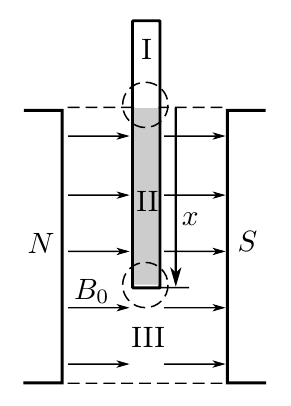
\includegraphics[width=\linewidth]{../res/rod.png}
	\caption{Стержень во внешнем магнитном поле.}
	\label{img:rod}
\end{wrapfigure}

Рассмотрим тонкий, длинный стержень, помещенный во внешнее однородное магнитное поле (рис. \ref{img:rod}). Магнитное поле в данной работе создаётся электромагнитом, для того чтобы оно было однородно площадь торцов электромагнита должна быть много больше размеров стержня, и стержень должен быть помещен в середину зазора.

В области $I$ магнитное поле пренебрежимо мало, в области $III$ оно примерно равно внешнему магнитному полю $B_0$. В области $II$ согласно рассматриваемой модели магнитное поле равно:
$$
\boldsymbol{B} = \chi \boldsymbol{H}
$$
На границах областей $I$ и $II$, $II$ и $III$ имеют место краевые эффекты, магнитное поле вычисляется сложно, поэтому чтобы ими можно было пренебречь стержень должен быть длинным.

С помощью метода виртуальных перемещений определим силу, действующую на стержень. Пусть длина области $II$ равна $x$, стержень имеет сечение $S$.

Определим поле внутри стержня. Вне стержня $B_0 = \mu_0 H_0$. Намагниченный внешним магнитным полем стержень будет вблизи создавать магнитное поле, так, что суммарное поле вблизи стержня в общем случае не будет равно внешнему магнитному полю. Для диа- и парамагнетиков $\chi \ll 1$, следовательно намагниченность стержня мала и поле вблизи него можно считать примерно равным внешнему магнитному полю. Тогда из непрерывности тангенциальной компоненты $H$ при переходе через границу находим, что напряженность внутри стержня $H_{ст} = H_0$, тогда $B_{ст} = \mu B_0$.

Определим объемную плотность энергии поля в диа- и парамагнетиках. Если $\boldsymbol{B} = \mu_0 \mu \boldsymbol{H}$, то объемная энергия поля равна:
$$
\omega = \int{\boldsymbol{H} d\boldsymbol{B}} = \frac{B^2}{2 \mu \mu_0}
$$

Рассмотрим бесконечно малое перемещение стержня на $dx$. Объем области $II$ увеличится на $S dx$, объем области $III$ уменьшится на $- S dx$. Тогда изменение энергии магнитного поля равно:
$$
\Delta W = \frac{B_2^2}{2 \mu \mu_0} S dx - \frac{B_3^2}{2 \mu_0} S dx = \chi \frac{B_0^2}{2 \mu_0} S dx
$$
Тогда искомая сила, действующая на стержень равна:
\begin{equation}
	F = \left( \frac{\partial W}{\partial x} \right)_{B_0} = \chi \frac{B_0^2}{2 \mu_0} S
	\label{theory:F}
\end{equation}
Из формулы (\ref{theory:F}) следуют, что парамагнетики втягиваются в зазор электромагнита, а диамагнетики выталкиваются.
